\documentclass{beamer}
\usetheme{Madrid}
% --- Packages requis pour ton code ---
\usepackage{tabularx}
\usepackage{booktabs}
\usepackage{tikz}
\usepackage{amsmath}
\usepackage{amssymb}

\begin{document}

% --- TON CODE COMMENCE ICI ---
\section{Comparison and takeaways}

\begin{frame}{Comparison: L0 vs L1/2 vs L1}
\small
\begin{tabularx}{\textwidth}{lXXX}
\toprule
 & \textbf{L0} & \textbf{L1/2} & \textbf{L1 (Lasso)} \\
\midrule
\textbf{Norm} & $\|\theta\|_0 = |\{i:\theta_i \neq 0\}|$ & $\|\theta\|_{1/2} = \sum_i |\theta_i|^{1/2}$ & $\|\theta\|_1 = \sum_i |\theta_i|$ \\[0.5em]
\textbf{Sparsity} & Very high (exact) & High (aggressive) & Medium/High \\[0.3em]
\textbf{Convex?} & No (discrete) & No ($p<1$) & Yes \\[0.3em]
\textbf{Optimization} & NP-hard (combinatorial) & Non-convex (ITA, MM) & Convex (proximal) \\[0.3em]
\textbf{Bias} & None (if found) & Low on large $\theta$ & Linear with $|\theta|$ \\[0.3em]
\textbf{Stability} & Very unstable & Sensitive to init. & Stable \\[0.3em]
\textbf{Complexity} & $O(2^p)$ exact & $O(n \cdot iter)$ & $O(n \cdot iter)$ \\[0.3em]
\textbf{Use-case} & Strict subset & Strong sparsity needs & General baseline \\
\bottomrule
\end{tabularx}
\end{frame}

\begin{frame}{When to use what?}
\begin{columns}[T,onlytextwidth]
  \begin{column}{0.32\textwidth}
    \begin{block}{Use L1 (Lasso)}
      \begin{itemize}
        \item ✓ Convex + reliable
        \item ✓ Fast solvers (LARS, proximal)
        \item ✓ Theory well-established
        \item ✓ Good baseline
        \item $\times$ Bias on large coefs
        \item $\times$ Moderate sparsity
      \end{itemize}
    \end{block}
  \end{column}
  
  \begin{column}{0.32\textwidth}
    \begin{block}{Use L1/2}
      \begin{itemize}
        \item ✓ Stronger sparsity than L1
        \item ✓ Less biased estimates
        \item ✓ Better signal recovery
        \item $\times$ Non-convex (local minima)
        \item $\times$ Needs good init.
        \item $\times$ Careful tuning
      \end{itemize}
    \end{block}
  \end{column}
  
  \begin{column}{0.30\textwidth}
    \begin{block}{Use L0}
      \begin{itemize}
        \item ✓ Optimal subset selection
        \item ✓ Maximal interpretability
        \item ✓ Unbiased 
        \item $\times$ NP-hard
        \item $\times$ Only small $p$ ($<$ 30-40)
        \item $\times$ Greedy approx needed
        \vspace{0.01cm}
      \end{itemize}
    \end{block}
  \end{column}
\end{columns}

\vspace{0.5em}
\centering
\textit{\footnotesize Practical tip: Start with L1, switch to L1/2 if you need more sparsity}
\end{frame}

\begin{frame}{Conclusion}
\begin{itemize}
  \item \textbf{L0:} Direct sparsity control, interpretable, but computationally intractable for large $p$. 
        \textit{Best for: feature selection with $p < 40$}
  
  \item \textbf{L1/2:} Bridges L0 and L1; achieves stronger sparsity with less bias than Lasso. 
        \textit{Best for: compressed sensing, medical imaging, signal reconstruction}
  
  \item \textbf{L1 (Lasso):} Industry standard—convex, stable, fast. 
        \textit{Best for: most real-world applications, production systems}
  
    
  \end{itemize}


    
\end{frame}
\begin{frame}
  \begin{itemize}
  \item \textbf{Key insight:} As $p$ decreases from 1 to 0, sparsity increases but optimization difficulty grows exponentially.
  
  \item Always balance the \textbf{trade-off triangle}:
\end{itemize}

\vspace{0.5em}
\centering
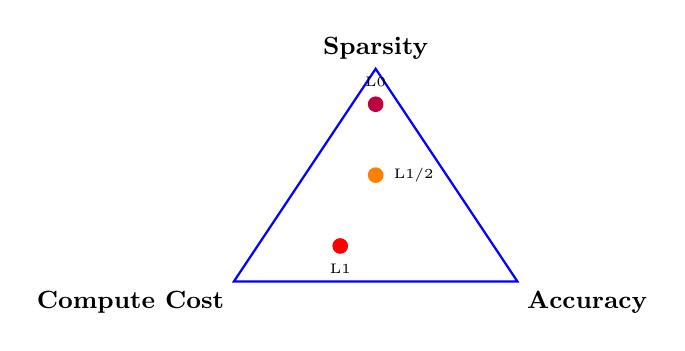
\begin{tikzpicture}[scale=0.9]
  \coordinate (A) at (0,0);
  \coordinate (B) at (4,0);
  \coordinate (C) at (2,3);
  \draw[thick,blue] (A) -- (B) -- (C) -- cycle;
  \node[below left,font=\small\bfseries] at (A) {Compute Cost};
  \node[below right,font=\small\bfseries] at (B) {Accuracy};
  \node[above,font=\small\bfseries] at (C) {Sparsity};
  
  % Positions des méthodes
  \node[circle,fill=red,inner sep=2pt,label=below:{\tiny L1}] at (1.5,0.5) {};
  \node[circle,fill=orange,inner sep=2pt,label=right:{\tiny L1/2}] at (2,1.5) {};
  \node[circle,fill=purple,inner sep=2pt,label=above:{\tiny L0}] at (2,2.5) {};
\end{tikzpicture}
\end{frame}

\begin{frame}{References}
\small
\textbf{Foundational papers:}
\begin{itemize}
  \item Tibshirani, R. (1996). \textit{Regression shrinkage and selection via the lasso}. JRSS-B.
  \item Xu, Z. et al. (2012). \textit{$L_{1/2}$ regularization: A thresholding representation theory}. IEEE Trans. Neural Networks.
  \item Bertsimas, D. et al. (2016). \textit{Best subset selection via a modern optimization lens}. Annals of Statistics.
\end{itemize}

\textbf{Books \& surveys:}
\begin{itemize}
  \item Hastie, T. et al. (2015). \textit{Statistical Learning with Sparsity} (Ch. 2-3).
  \item Mallat, S. (2008). \textit{A Wavelet Tour of Signal Processing} (Sparse representations).
\end{itemize}

\textbf{Software:}
\begin{itemize}
  \item \texttt{scikit-learn} (Lasso, ElasticNet), \texttt{L0Learn} (R package), \texttt{CVXPY} (convex optimization)
\end{itemize}
\end{frame}

% --- FIN DE TON CODE ---
\end{document}
